% Author: Anachuri Nicolas Daniel Template for myself
 
%\documentclass[11pt]{article}
\documentclass[11pt]{article}

\usepackage{indentfirst} 		% First line paragraph indentation
\usepackage{etoolbox} 			% Used for being able to utilise if statements in the language detection.
\setlength{\parskip}{\baselineskip}	% With this line, it is not needed the use of \\ at the end of each paragraph for spacing purposes


% ========================= VARIABLES TO MODIFY =================================

\def\LANGUAGE{EN} %EN, ES		%Language in which the document is going to be written.

\def\reportTile{Fisica Aplicada}			%Document's title
\def\subject{Trabajo Practico N.1}			%Subject

\def\writter{Anachuri Nicolas Daniel y Tito Benjamin Emanuel}		%Author(s)


\def\leftUpperHeader{\subject}		%\subject
\def\rightUpperHeader{\leftmark}	%\leftmark for current section


% Do NOT modify anything from here until the beginning of the document.
%============================== DATA PROCESSING ============================
\ifdefstring{\LANGUAGE}{EN}
{

\def\course{1ro del Superior Informatica} %---------
\def\university{Escuela de Minas Dr. Horacio Carrillo} %------------
\def\pageCounterName{PAGE} 		% In the footer will be shown this... 
\def\pageSeparator{OUT OF} 		% ...text in addition of the page number.

}
{
\usepackage[utf8]{inputenc}		%Tildes en caso de no usar arch
\usepackage[spanish, es-tabla]{babel} 	%La opción es-tabla, hace que por defecto las tablas se llamen "Tabla", en vez de "Cuadro".
\def\course{1ro del Superior Informatica} %----------
\def\university{Escuela de Minas Dr. Horacio Carrillo}
\def\pageCounterName{PÁGINA}		%En el pie de página aparece este contenido más el número de página
\def\pageSeparator{DE} 			%DE, OUT OF

}


%===================== USEFUL VARIABLES  =============================
\def\imageSize{0.9}

%===================== PACKAGES TO USE  =============================
\usepackage{amsmath} 			% Allows me the use of matrix in math mode
\setcounter{MaxMatrixCols}{20} 		% Increases the maximum number of columns in matrix from 10 to 20.
\usepackage{pdfpages} 			% Attach pdfs using \includepdf[pages=initial-final]{path.pdf}
\usepackage{lastpage}			% Used to reference the last page and include it in the footer.
\usepackage{xcolor}			% Change color of text and so on. \textcolor{color}{text} is the one I use the most.
\usepackage{placeins} 			% Allows the use of the command \FloatBarrier
\usepackage{setspace}			% Allows the use of the spacing environment to change the space between lines.
\usepackage{graphicx}			% Figures addition
\usepackage{wrapfig}
\usepackage{geometry}			% Changes the geometry of the pages
\usepackage[small, bf]{caption}		% Decreases the size of captions and turns them bold text.
\usepackage{subcaption}			% Include subfigures.
\usepackage{hyperref}			% Allows clickable references.
\hypersetup{colorlinks=true, allcolors=black} 	% Colors of links
\usepackage{pdflscape}			% Allows the use of the environment lscape for landscape pages
\usepackage{filecontents}
\usepackage{fancyhdr}			% Modify header and footer
\usepackage{bm}				% Allows to use bold text in math mode with \bm
\usepackage[makeroom]{cancel}		% Allows the use of \cancelto{}{} to cross out equations
\usepackage{titlesec}			% Change title format
\usepackage{filecontents}
\usepackage{glossaries}
%========== CHANGE TITLE FORMAT  ======================
%\titleformat{\section}
%{\bfseries}	% format
%{\thesection}	% label
%{0.3cm}		% separation between label and body
%{}		% code preceding title body
%[]		% code following title body


%========== HEADER AND FOOTER CONFIGURATION ======================
\pagestyle{fancy}
% HEADER[EVEN PAGES]{ODD PAGES}
% Left header
\lhead[
	\scriptsize{\MakeUppercase{\leftUpperHeader}} % Even pages
]
{
	\scriptsize{\MakeUppercase{\leftUpperHeader}} % Odd pages
}

% Central header
\chead[]{}

% Right header
\rhead[
\scriptsize{\rightUpperHeader} % Even pages
]
{
\scriptsize{\rightUpperHeader} % Odd pages
}

\renewcommand{\headrulewidth}{0.8pt}	% Width of the header rule

% FOOTER[EVEN PAGES]{ODD PAGES}
% Left footer
\lfoot[]{}

% Central footer
\cfoot[
\tiny{\pageCounterName\space\thepage\space \pageSeparator\space\pageref{LastPage}} % Even pages
]
{
\tiny{\pageCounterName\space\thepage\space \pageSeparator\space\pageref{LastPage}} % Odd pages
}

% Right footer
\rfoot[]{}
\renewcommand{\footrulewidth}{0.8pt} %Width of the footer rule


%================================== USER OWN FUNCTIONS ===============================================
\newcommand{\PDEA}[1]{\cdot 10^{#1}} % Función para escribir más rápidamente multiplicaciones por potencias de 10. PDEA = Por Diez Elevado A

\usepackage{xargs}	%Permite manejar argumentos opcionales en los comandos creados por el usuario

%Incluir imágenes, la sintaxis es la siguiente:
%\IncludeImage{ruta}[escalado][pie figura][etiqueta], los corchetes son opcionales
\newcommandx*{\IncludeImage}[4][2=1, 3=, 4=]{
	%#1 es la ruta a la imagen
	%#2 es el escalado
	%#3 es el pie de figura
	%#4 es la etiqueta
	
	\begin{figure}[h!]
		\centering
		\includegraphics[width=#2\linewidth]{#1}
		%Si se especifica pie de figura...
		\ifblank{#3}{}{
			\caption{#3}	
		}
		%Si se especifica etiqueta...
		\ifblank{#4}{}{
			\label{#4}	
		}
	\end{figure}
	\FloatBarrier
}
% ========================== GLOSSARIES ===================================

\makeglossaries

\newglossaryentry{empirico}
{
    name=Empirico,
    description={Informacion recibida por  medio de los sentidos, particularmente la observacion}
}

\newglossaryentry{duras}
{
    name=Ciencias Duras,
    description={Ciencias Basadas enteramente en la observacion y experimentacion}
}
\newglossaryentry{todo}
{
    name=Ciencias Teoria del Todo,
    description={sugiere que el universo evoluciona según leyes bien definidas}
}
\newglossaryentry{radiacion}
{
    name=Radiacion de Hawking,
    description={Según Hawking, los efectos de las física cuántica hacen que los agujeros negros brillen como cuerpos calientes, de ahí que pierdan parte de su negritud.}
}




%================================ DOCUMENT BEGINNING  =============================================
\begin{document}
%***************** TITLE PAGE (DO NOT MODIFY) ******************************
\begin{titlepage}
	\newgeometry{top=2cm, bottom=3.5cm}

	%Logos Escuela y universidad
	\def\logoSize{0.2}
	\begin{figure}
	\includegraphics[width=\logoSize\linewidth]{/home/nico/Descargas/minas.jpeg}
	\hfill
	\includegraphics[width=\logoSize\linewidth]{/home/nico/Descargas/unju.jpeg}
	\end{figure}


	%Espacio entre logos y título
	\vspace*{1.75cm}

	%Título con interlineado aumentado
	\begin{spacing}{2}
	\centering{
	\Huge{
		\textbf{\reportTile}
	}
	}
	\end{spacing}
	
	%Línea horizontal de la portada
	\hrule
	
	%Se baja al final de la hoja
	\vfill
	\begin{flushright}
	\LARGE{\writter}

	\vspace{2cm}
	
	\Large
	\subject\\
	\course\\
	\university
	
	\vspace{1cm}
	
	\today
	\end{flushright}
	
\end{titlepage}
	
\newgeometry{top=3cm, bottom=3cm}

\tableofcontents
%\cleardoublepage
\clearpage


\section{Metodo Cientifico:}

%Es primordial en la investigacion de las ciencas duras, El metodo cientifico fue implantado primeramente por Galileo Galilei durante $XVII$ a mediados del $XVIII$, Vivio en la era del Renacimiento , Astronomia , Rotacion sobre su eje de la tierra, Direccion de movimiento de los planetas y descubrimiento de las orbitas. El método científico es una metodología para obtener nuevos conocimientos, que ha caracterizado históricamente a la ciencia, y que consiste en la observación sistemática, medición, experimentación y la formulación, análisis y modificación de hipótesis. Las principales características de un método científico válido son la falsabilidad, y la reproducibilidad y repetibilidad de los resultados, corroborada por revisión por pares\cite{coper}.

El método cientifico es apropiado para el estudio de las \gls{duras}. Se considera a Galileo Galilei entre los siglos $XV - XVI$ mas precisamente (1564-1642) como el padre del método científico. Fue un físico y astrónomo que propició la revolución científica durante el Renacimiento. Algunos de sus aportes son la mejora del telescopio, el compás geométrico, el estudio del movimiento del péndulo y el descubrimiento de las lunas de Júpiter.

\begin{wrapfigure}{l}{0.6\linewidth}

  \centering
  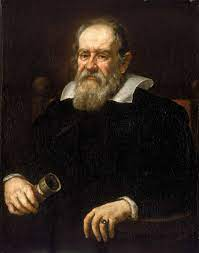
\includegraphics[width=0.6\linewidth]{/home/nico/me/Fisica/TP2-AnachuriNicolas-TitoBenjamin/galileo.jpeg}
  \caption{Galileo Galilei}
  \label{fig:etiqueta}

\end{wrapfigure}

El \textbf{Metodo Cientifico} \cite{historia} es un metodo \gls{empirico} para la adquisicion de conocimiento que ha caracterizado  el desarrollo de la ciencia, el cual involucra la observacion y el escepticismo sobre lo que es observado. La formulacion de una \textbf{Hipotesis} via induccion. La \textbf{Experimentacion} que aporta deducciones. Los \textbf{Resultados} dado por los experimentos para el refinamiento (o su eliminacion) de la hipotesis. Y \textbf{tiene} que ser repicable para cualquier otra persona.

%2.- Describa el campo de estudio\cite{notes} de la FISICA como ciencia (tres renglones).

\section{Campo de estudio de la Fisica}

La \textbf{física} es la ciencia natural que estudia los componentes fundamentales del Universo, la energía, la materia, el espacio-tiempo y las interacciones fundamentales.

\section{Materia}

\subsection{Estados de la Materia}
\begin{itemize} 
  \item Solido 

  \item Liquido

  \item Gaseoso 

  \item Plasmatico
    
  \item Condensado de Bose-Einstein
    
  \item Condensado de Fermi

  \item Superfluido
  
  \item Supersolido 
  
  \subsection{Tipos de cambio de estado}
  
  \item Fusión: Es el pasaje de un sólido a líquido por medio de exposición al calor. Ej: la fundición de los metales en hornos.
  \item  Solidificación: Es el pasaje de líquido a sólido por medio del enfriamiento. Ej: Formacion del Hielo
  \item  Vaporización y Ebullición: Son los procesos en los que la materia pasa del estado líquido al estado gaseoso. Ej: Hervir Agua.
  \item  Condensación: Es el pasaje de gaseoso a líquido. Ej: Descongelamiento del Hielo.
  \item Sublimación: Es el pasaje del estado sólido al estado gaseoso sin pasar por el estado líquido. Una sustancia capaz de sublimarse es el hielo seco. Ej: el hielo seco (dióxido de carbono seco).
  \item  Sublimación inversa: Es el pasaje directo del estado gaseoso al sólido, sin pasar por el estado sólido. Ej: Formación de la nieve 
  \item  Ionización: Es el cambio de un gas a un plasma. Ej: Inonización por electrones
  \item  Desionización: Es el cambio de un plasma a un gas. Ej: la disolución de la sal de mesa en el agua.
\end{itemize}



%3.- si decimos que la física y la química estudian la materia, entonces pregunto a) cuales son los estados de la materia? b) como se denominan los cambios de estado de la materia. Podrían citar un ejemplo en cada uno de ellos.


\section{Magnitudes}

Las \textbf{magnitudes} pueden ser clasificadas de acuerdo a a su expresión matemática y según su actividad. Según su expresión matemática puede clasificarse en escalares, vectoriales y tensoriales. Según su actividad, se clasifican en extensivas e intensivas.

\section{Sistema de Unidades}

% sistema de unidades de longitud, de masa y de tiempo. Que entendemos por sistema de unidades: ¿MKS, CGS, TÉCNICO O PRÁCTICO?

\subsection{Sistema de Longitud}

Una unidad de Longitud\cite{longitud} es una cantidad estandarizada de longitud definida por convención. La longitud es una cantidad básica creada para medir la distancia entre dos puntos.  Existen varios sistemas de unidades para esta cantidad física. Los más utilizados son el Sistema Internacional de Unidades y el Sistema de Unidades Anglosajón.

\subsection{Sistema de Masa}

Es una magnitud física y propiedad general de la materia, que expresa la inercia o resistencia al cambio de movimiento de un cuerpo. De manera más precisa es la propiedad de un cuerpo que determina la aceleración del mismo, cuando este se encuentra bajo la influencia de una fuerza dada. Es una propiedad intrínseca de los cuerpos que determina la medida de la masa inercial y de la masa gravitacional. La unidad utilizada para medir la masa en el Sistema Internacional de Unidades es el kilogramo $Kg$.


\subsection{Sistema de Tiempo}

El tiempo es una magnitud física creada para medir el intervalo en el que suceden una serie ordenada de acontecimientos. El sistema de tiempo comúnmente utilizado es el calendario gregoriano y se emplea en ambos sistemas, el Sistema Internacional y el Sistema Anglosajón de Unidades. 

\subsection{MKS}


Se basa en unidades de $longitud$, $masa$ y $tiempo$. La sigla MKS hace referencia, justamente, a las palabras metro, kilogramo y segundo. Las longitudes son medidas en metros, la masa es medida en kilogramos y el tiempoen segundos. Esto es bastante útil para medir magnitudes cuyas dimensiones suelen ser grandes, como por ejemplo el ancho de una casa, la altura de una jirafa o la masa de una ballena.

\subsection{CGS}

El sistema CGS es el otro de los sistemas de medida basados en $longitud$, $masa$ y $tiempo$. Sin embargo, la sigla CGS hace referencia a las palabras centímetro, gramo y segundo. Es útil es para medir magnitudes cuyas dimensiones son pequeñas, tales como el ancho de tu celular, la masa de una lombriz o la energía del aleteo de una mariposa.

\subsection{Tecnico}

Se diferencia radicalmente de los dos anteriores en que sus magnitudes fundamentales ya no son la longitud, la masa y el tiempo, sino que lo son la $longitud$ , $peso$ y $tiempo$.  Sus unidades fundamentales son el metro, el kilogramo-fuerza y el segundo. Utiliza el kilogramo-fuerza como unidad fundamental.

\section{Cientificos}

\subsection{Cientificos de la Antiguedad} 

\begin{itemize}
  \item  Arquímedes: Creó numerosas herramientas revolucionarias para la historia de las matemáticas, como la palanca o el tornillo de Arquímedes y dió una aproximación extremadamente precisa del número pi.
  \item Nicolás Copérnico: Formuló la teoría heliocéntrica del sistema solar.
  \item  Leonardo Da Vinci: desarrolló ideas muy adelantadas a su tiempo, tales como el helicóptero, el carro de combate, el submarino y el automóvil. Como científico, hizo progresar mucho el conocimiento en las áreas de anatomía, la ingeniería civil, la óptica y la hidrodinámica.
\end{itemize}

\subsection{Cientificos del Siglo $XX$}
\begin{itemize}
  \item Albert Einstein\cite{einstein}: Teoria de la Relatividad GeneralTeoría de la relatividad especial, El efecto fotoeléctrico, Ecuación E=MC²,  Teoría de la relatividad general, Teoría de campo unificado. ... 
  \item Alan Turing: Formalizó los conceptos de algoritmo y computación con su máquina de Turing. Es considerado el padre de la inteligencia artificial. Su participación en el equipo de criptoanálisis de la máquina de criptografía alemana Enigma fue clave
  \item Stephen Hawking:  aporto a la investigacion de los agujeros negros, \gls{radiacion} , \gls{todo} 
\end{itemize}

\begin{thebibliography}{100}
    
\bibitem{historia} Peter Achinstein, General Introduction (pp. 1-5) to Science Rules: A Historical Introduction to Scientific Methods. Johns Hopkins University Press, 2004. ISBN 0-8018-7943-4

\bibitem{Galileo} Robin Santos Doak, Galileo: Astronomer and Physicist, Capstone, 2005, p. 89.
  
\bibitem{einstein} https://en.wikipedia.org/wiki/Albert_Einstein

\bibitem{fisica} https://es.wikipedia.org/wiki/F%C3%ADsica
  
\bibitem{Estados} https://es.wikipedia.org/wiki/Estado_de_agregaci%C3%B3n_de_la_materia
  
\bibitem{magnitud} https://es.wikipedia.org/wiki/Magnitud_f%C3%ADsica
  
\bibtiem{copernico} https://es.wikipedia.org/wiki/Nicol%C3%A1s_Cop%C3%A9rnico


\section{Profesor Elegido}

Nuestro profe elegido ..... ........  es bastante tranquilo, mantiene la voz baja, a excepcion de cuando quiere explicar, es amigable pero no es de hablar con otros profesores,   trabaja en el ciclo bajo y superior ,fisicamente es rellenito ,usa lentes, siempre lleva un maletin, tiene estatura promedio-baja, es el encargado del equipo de olimpiadas, Le gustan los juegos. Da clases en la facultad de ingenieria  


\end{thebibliography}

\printglossary





\end{document}



